\chapter{The exploration of self-organisation via contribution activities: conceptualising Drupal through an Activity Theory lens}
\chaptermark{Activity Theory}
\label{sec:theoretical-frameworks}

This chapter presents an overview of the case study conceptualised through Activity Theory, the main theoretical framework employed for this research. Rather than a theory in the strict sense, Activity Theory is an analytical tool, a lens that helps researchers and practitioners to analyse complex activities, such as in Free\slash Libre Open Source Software as part of the wider phenomenon of Commons-Based Peer Production.

Firstly, a summary of Activity Theory will be presented in section \ref{subsec:at}, providing a historical overview of the three different generations of Activity Theory, the main theoretical concepts underpinning it, its limitations and discussions of activity theorists about it. Secondly, section \ref{subsec:why-at} offers a summary of the reasons why Activity Theory has been chosen for the study of peer production. Finally, section \ref{subsec:at-conceptualisation} provides a detailed explanation of the process carried out to analyse the activities involved in Drupal, drawing on the main concepts of Activity Theory, as well as a set of practical examples of its application to the case study.

\section{A historical overview of Activity Theory}
\label{subsec:at}

\subsection{Historical roots and the first generation}

The historical roots of Activity Theory (AT) can be found in classical German philosophy, from Kant to Hegel, as well as in the work of Marx and Engels. In ``\textit{Theses on Feuerbach}", \textcite[143-45]{marx1845theses} defined the idea of object-oriented activity and discussed the relationship between object and subject during production. According to Marx, the subject produces itself by producing the object while transforming the object's nature. The process is understood as a historical phenomenon, which is dependent on social practices. Another important influence of classical Marxism in AT is the concept of inner contradictions within the system, which can result in a force of development \parencite{hegel1861lectures}.

The main theoretical pillars of AT started being developed in the 1920s, and can be traced within the Soviet cultural-historical psychology field pioneered by Vygotsky, Leont'ev and Luria \parencite{engestrom1999activity}. A key concept is that of mediated action proposed by \textcite{vygotsky1978mind} as an alternative to the behaviourist views on human activities at the time. According to Vygotsky, human action is mediated by culturally meaningful artefacts. By collaborating in the development of activities with other humans, the meanings, social norms and modes of acting are internalised by the individual. This relationship between the subject, the object and the cultural means, norms and signs proposed by Vygotsky, is usually represented as a triangle (see figure \ref{vygotsky-first-gen}), in which the artefacts also embed some of these cultural properties.

\begin{figure}[H]
	\centering
	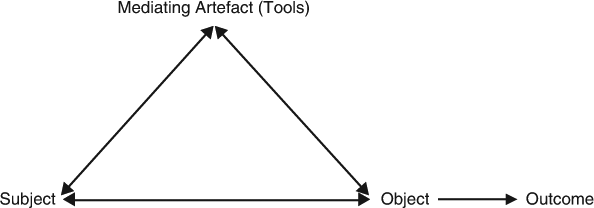
\includegraphics[scale=0.6]{img/vigotsky_first_gen.png}
	\caption[Vygotsky's model of mediated action]%
	{Vygotsky's model of mediated action: the first generation. \textcite{flavin2012disruptive}.}
	\label{vygotsky-first-gen}
\end{figure}

As in the case of other socio-cultural perspectives \parencite{kaptelinin2012}, this model assumes the social nature of the human mind, as well as its inseparability from the activity. Thus, activities are influenced by the characteristics of the subjects and the objects, and vice versa. For instance, as exemplified by \textcite{kaptelinin2012}, whether a mathematical problem can be solved by a certain subject depends on the characteristics of the object, for example how hard the mathematical problem is. It is also dependent on the characteristics of the subject, for example the subject's mathematical skills. The subject's skills in mathematics are influenced by its previous experience in solving mathematical problems. Hence, while the subject's abilities influence solving the mathematical problem, solving mathematical problems will also influence the subject's abilities over time, for example, improving their knowledge and skills. Therefore, over time, the object and the subject are transformed by the activity, and subjects are also produced by the activities \parencite{kaptelinin2012}.

Subsequently \textcite{leontjev1978activity}, as part of a reaction against the work of Vygotsky, developed the notions of mediated social processes and established the concept of activity as an unit of analysis. This definition of the collective activity system as unit of analysis allowed the connection between psychological, organisational and cultural approaches. Hence, rather than focussing exclusively on the individual as in previous approaches, the interactions between the subject, the artefacts and other individuals under certain organisational settings can be explored. In addition, he distinguished between the concepts of activity, action and operation (see figure \ref{leontiev-three-level-model}) and developed them in a more precise manner:

\begin{itemize}
	\item \textit{Activity}: a set of actions and operations, defined by motives and driven by an object. They are typically long time affairs.
	\item \textit{Action}: they are focussed on goals, conscious and tool-mediated processes.
	\item \textit{Operation}: they are the methods for accomplishing actions. They are routine cognitive or behavioural processes, subject to the conditions of the system.
\end{itemize}

\begin{figure}[H]
	\centering
	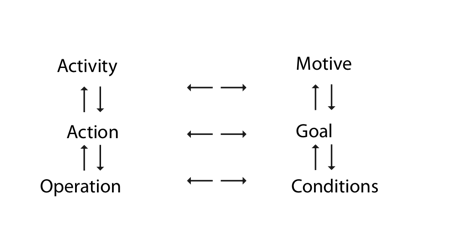
\includegraphics[scale=1.2]{img/leontiev_three_level_model.png}
	\caption[Leont'ev's three-level model]%
	{\textcite{leontyev1981outline} three-level model.}
	\label{leontiev-three-level-model}
\end{figure}

For instance, as exemplified by \textcite{kaptelinin2012}, an activity can be learning how to drive a car, and the motives for a subject could be to obtain a driving license to apply for a job. As an activity, learning how to drive is composed of actions, which are conscious processes directed at goals. For example, the subject may decide to register in a driving school or to arrange some practical sessions, which are examples of actions. Actions are then carried out through operations, which are oriented towards the conditions of the subject to meet the goals. For instance, shifting gears during a practical session. Subjects are typically not aware of their operations, although they can be during the process of internalisation. For example, the operation of shifting gears will typically be transformed from a conscious action into a routine one, without needing conscious control, over the course of the activity of learning how to drive a car.

\subsection{The second generation}
\label{subsec:2at}

In the 1980s, AT started being studied in academic environments out of the Soviet Union. \textcite{engestrom1987learning} proposed an extension of Leont've's model adding three new elements: the rules that regulate the activity, the community sharing the interest and the division of labour (see figure \ref{engestrom-diagram-sec-gen}). The relevance of some of these elements was already signified by activity theorists from the first generation. For example, in Leont'ev's classical example of hunting as a collective activity, he drew on the notion of division of labour to explain why the actions of a group might be motivated by an object although they might be directed at a different one \parencite{nardi2006activity}. For instance, a group of hunters can divide themselves into two groups: the first group shakes the bushes to scare the animals in a specific direction, while the other group waits to hunt them. Their motivation might be the same, for instance taking part in the hunt as part of their contribution to the hunting activity, but their immediate goals in this example were different: for the first group it was scaring the animals, while for the second one it was killing them.

Overall, the work of the second generation of activity theorists highlighted these social aspects and developed the theoretical tools to conceptualise them. For example, Engestr{\"o}m proposed a new unit of analysis, the \textit{human activity system}, which extended Leont'ev's as follows \parencite{Foot2001}:

\begin{itemize}
	\item It is dynamic, instead of static
	\item It represents the complexity of the whole
	\item It is specific to human beings, by being culturally mediated
	\item It is analysable in its context.
\end{itemize}

In addition, Engestr{\"o}m proposed a new model for the theoretical framework usually represented as a triangle with six interrelated elements and the outcome of the activity (see figure \ref{engestrom-diagram-sec-gen}). In this model, which has been known as that of the second generation of AT, the elements can be understood as follows:

\begin{itemize}
	\item \textit{Subject}: the actors who perform the activity and who are subject to the internalisation processes.
	\item \textit{Mediating artefacts}: the tools employed by the actors in the system. They have an influence on the actors and on the structure. They are also influenced by the culture, and change according to the accumulated experience.
	\item \textit{Object}: the element towards which activity is directed. It is transformed as the activity progresses and it possesses social and cultural properties.
	\item \textit{Rules}: they are the explicit and implicit rules which regulate the activity in the system.
	\item \textit{Community}: they are all of the actors involved in the system.
	\item \textit{Division of labour}: a representation of the distribution of processes between the actors of the system.
\end{itemize}

\begin{figure}[H]
	\centering
	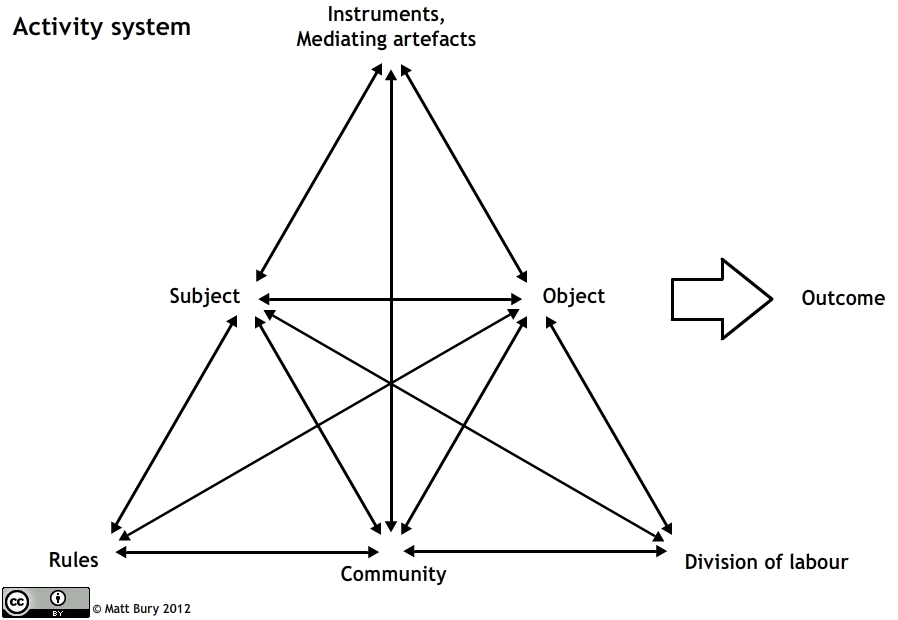
\includegraphics[scale=0.3]{img/engestrom_diagram.png}
	\caption[Engestr{\"o}m's activity system diagram]%
	{Engestr{\"o}m's activity system diagram. Matt Bury (2012), under a CC BY-SA 3.0.}
	\label{engestrom-diagram-sec-gen}
\end{figure}

For instance, as epitomised by \textcite{kaptelinin2012}, an activity could consist of the redesign of the user interface of a computer application, in which the object of the activity is the current interface. The community is formed by the members of the team working on the redesign, which involves a division of labour (e.g. project managers, developers and user interface designers). An interface designer might use a set of arterfacts to work on the transformation of the object, ranging from physical objects such as computers, to other software applications for designing and implementing changes. This interface designer might establish different interactions with the community through implicit and explicit rules, for example attending project meetings or receiving a salary for the work. Overall, the coordinated work of the team produces a set of new outcomes, such as that expected of the new user interface.

Although, as previously discussed, Leont've's work mentioned that activities are not only carried out by individuals but also by collectives, the first generation of Activity Theory did not present a conceptual model for the study of collective activities as seen in the previous example \parencite{kaptelinin2012}. Thus, the work of the second generation of activity theorists, and most prominently Engestr{\"o}m, developed the theoretical tools and extended the model in order to address some of the limitations of the first generation of Activity Theory. 

\subsection{The third generation and beyond: Activity Theory for the study of organisational forms in the network society}
\label{subsec:3at}

The increase in complexity of some of the phenomena to be studied, such as complex systems represented by networks for which the model of a single activity system was insufficient, produced a debate between activity theorists in the 1990s. \textcite{engestrom199923} proposed an extension of the second generation AT framework to capture interactions between several human activity systems. Figure \ref{engestrom-diagram-third-gen-a} depicts the minimal model, with two interacting activity systems. As a result, objects shared between several systems are constructed and can be studied. In addition, the contradictions, interactions and tensions between several systems are also seen as a possible force of development.

\begin{figure}[H]
	\centering
	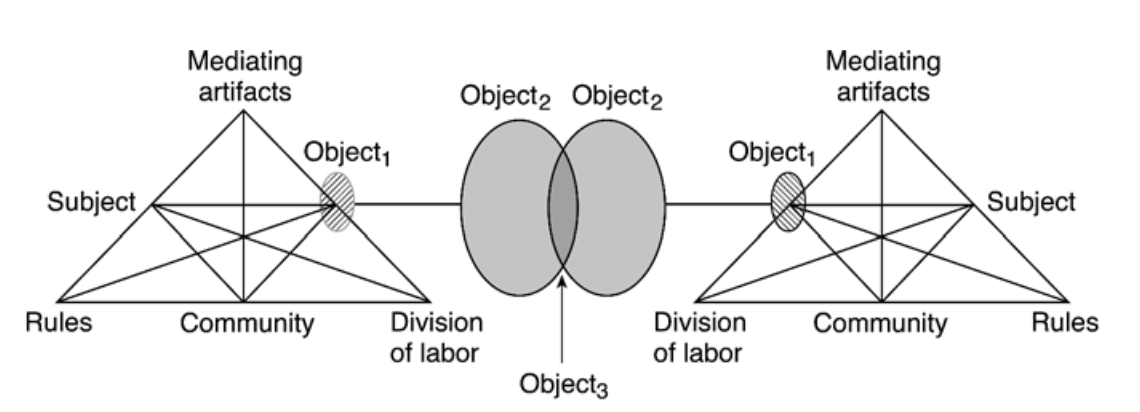
\includegraphics[width=\textwidth]{img/engestrom_shared.png}
	\caption[Engestr{\"o}m's third generation model]%
	{Engestr{\"o}m's third generation model. \textcite[136]{engestrom2001}.}
	\label{engestrom-diagram-third-gen-a}
\end{figure}

For instance, continuing with the previous example of the activity to redesign the user interface of a computer application \parencite{kaptelinin2012}, this new user interface --- the main expected outcome --- could be part of a larger effort for developing a new version of the whole application, requiring the integration of the outcomes from other activity systems.

Furthermore, in the last decade the emergence of new forms of organisation, such as Commons-Based Peer Production, distributed work or co-working, opened a debate between activity theorists on the need to rethink the shape of these activity systems \parencite{engestrom_future_2009}. The discussion was initiated by \textcite{engestrom-myco} when drawing on a mycorrhizae metaphor while establishing a comparison with the well-known concept of ``community of practice"  \parencite{wenger1998communities}. With this, he provided an initial account of the characteristics of some of these new forms of organisation \parencite[51-52]{engestrom-myco}:

\begin{quotation}
 ``Mycorrhizae are difficult if not impossible to bound and close, yet not
indefinite or elusive. They are very hard to kill, but also vulnerable.
They may lie dormant for lengthy periods of drought or cold, then
generate again vibrant visible mushrooms when the conditions are
right. They are made up of heterogeneous participants working
symbiotically, thriving on mutually beneficial or also exploitative
partnerships with plants and other organisms. [...]

A mycorrhizae formation is simultaneously a living, expanding
process (or bundle of developing connections) and a relatively
durable, stabilized structure; both a mental landscape and a material
infrastructure.''

\end{quotation}

Drawing on this metaphor, Engestr{\"o}m introduced in the debate \parencite{engestrom2006well} and subsequently developed \parencite{engestrom_future_2009} the concept of \textit{runaway object}. The term was inspired by the concept of \textit{runaway world} originally coined by \textcite{giddens2011runaway} in his work focussed on the implications of global capitalism, such as lack of control. Drawing on this concept, \textcite[98]{ciborra2002labyrinths} provides an account of the characteristics of this lack of control of global phenomena, such as global warming:

\begin{quotation}
 ``We experience control in the age of globalization as more limited than ever. We are creating  new  global  phenomena  (global  warming  and  greenhouse  effects, nuclear  threats, global production processes, and so on) that we are able to master only in part. Although information infrastructures appear to be important instruments for governing global phenomena, they possess ambiguities which make their eventual outcome difficult to determine.''

\end{quotation}

Drawing on these notions, \textcite{engestrom2006well} aimed to capture, among other aspects, the less clear boundaries and structures of activity systems in cases such as peer production that imply a continuous challenge for the use of theoretical frameworks, from which AT is not an exception. To that end, Engestr{\"o}m unbounded the concept of object in Activity Theory \parencite{spinuzzi2011losing}, expanding this key notion to update the AT framework in order for it to remain a useful lens for the study of phenomena under the expansion of global capitalism, in which these objects ``have the potential to escalate and expand up to a global scale of influence. They are objects that are poorly under anyone's control and have far-reaching, unexpected side effects" \parencite[227]{engestrom2008teams}. As examples, \textcite{engestrom_future_2009} includes global warming, but also ``benign" runaway objects which can be ``powerfully  emancipatory objects that open up radically new possibilities of development and well-being, as exemplified by the Linux operating system" \parencite[1784]{engestrom2006well}.


In his subsequent work \textcite{engestrom_future_2009} made more concrete the characteristics of these benign runaway objects, drawing on other well-known examples of Commons-Based Peer Production, such as Wikipedia, other FLOSS communities beyond GNU/Linux, organic farming or open research and publishing among others. Firstly, \textcite[306]{engestrom_future_2009} provided a more accurate set of prerequisites of what runaway objects are:

\begin{itemize}
	\item They must have intrinsic properties that transcend the utilitarian profit motive
	\item The object must yield useful intermediate products, yet remain an incomplete project
	\item The object must be visible, accessible and cumulable
	\item There must be effective feedback from and exchange among the participants acting on the object.
\end{itemize}

Secondly, \textcite[314-317]{engestrom_future_2009} highlighted the notions of negotiation and peer review as key to understand the nature of the object and the coordination mechanisms of these new forms of organisation, such as in the case of Drupal. Figure \ref{engestrom-diagram-third-gen-b} depicts this new model, in which it is acknowledged and highlighted that the boundaries and structures in these new forms of organisation, such as peer production, are not so clear: they are subsumed by the object, rather than the other way around.

\begin{figure}[H]
	\centering
	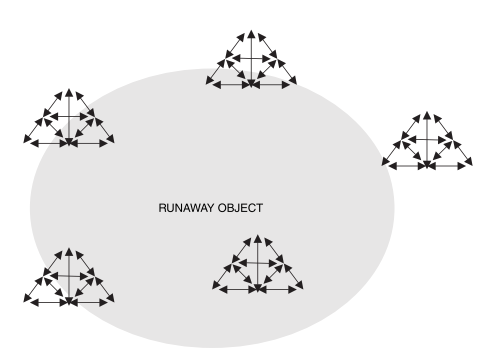
\includegraphics[scale=0.5]{img/engestrom_third_gen_b.png}
	\caption[Engestr{\"o}m's third generation model for runaway objects]%
	{Engestr{\"o}m's third generation model for runaway objects. \textcite[306]{engestrom_future_2009}.}
	\label{engestrom-diagram-third-gen-b}
\end{figure}

This third generation of AT is under ongoing discussion amongst activity theorists. For example, \textcite{roth2007emotion} proposes the inclusion of emotions and their interactions with respect to other entities as part of the role they play in mediated actions; or \textcite{spinuzzi2011losing} criticises the excessive expansion of the concept of object, and argues to contract it instead, proposing five counter-movements for a methodological and theoretical contraction applicable for each specific case study.

Nevertheless, there is a high degree of consensus between activity theorists in acknowledging that the ongoing changes in the new forms of organisation, such as Commons-Based Peer Production, are so profound that they require a radical rethinking of the models, in what could be considered as an emerging fourth generation of Activity Theory \parencite[306-310]{engestrom_future_2009}. Indeed, some of the most recent work of Engestr{\"o}m, as well as that of other scholars, in which Activity Theory is employed for the study of these rapidly changing forms of organisation, such as peer production, non-employer firms, distributed work or co-working to name but a few, is tackling some of these challenges \parencite[e.g.][]{engestrom2016using, spinuzzi2014nonemployer, dochy2011inter}. Overall, this can be interpreted as a shift in the focus from the inner workings of the human activity system towards the interactions and connections which these activity systems form. Hence, this shift in focus allows the conceptualisation of these systems and the interactions and connections between them as networks, as a response to the rapid changes in organisation experienced in the network society, as argued by \textcite{castells2011rise}, among many other proponents.

As it will be discussed in section \ref{subsec:at-conceptualisation}, a similar challenge emerged when employing AT as a theoretical framework for the conceptualisation of the case study in this research, which was tackled using a new definition of a concept connecting these activity systems within the context of Commons-Based Peer Production which was inspired by the work of the aforementioned scholars.

\section{Why draw on Activity Theory for the study of peer production?}
\label{subsec:why-at}

During the design of this research, other theoretical approaches, such as social practice theory \parencite{shove2012dynamics} or Actor-Network Theory \parencite{latour1987science, callon1986some} were evaluated and considered less adequate than AT. For example, with regard to the former, due to a less extensive application for the study of socio-technical systems, including online communities, with respect to AT and Actor-Network Theory. Regarding the latter, Actor-Network Theory and Activity Theory possess a set of common characteristics \parencite{miettinen1999riddle}, such as avoiding monocausal explanations, sharing some social constructivist principles, being built on top of the object-oriented idea of Marx, remarking the importance of the artefacts and their meanings, and studying the networks of actors among others. However, both approaches present important differences in their conceptual formulation. For example, one of the central notions in Actor-Network Theory is that of an \textit{actant}, which establishes that both human and non-human elements of the network should be given the same kind of treatment. This is also reflected, for example, in a symmetrical interpretation of the mediation. In contrast, AT proposes a dialectical and asymmetrical interpretation of the mediation, in which some of the entities, such as the subject, possess a different capacity to build associations, more fitting for the context of this case study. In addition, Actor-Network Theory ignores processes such as learning, development of expertise and know-how in network construction \parencite{miettinen1999riddle}. All these elements, which emerged as relevant from the beginning of this study, are included in AT. Additionally, as previously presented, AT provides a more concrete model for the study of the relationships between all of these different elements, and includes the notion of tensions as a conceptual element for the study of these systems. These elements also emerged as key from the beginning of this study in order to conceptualise the nature of peer production activities.

Rather than as a theory in the traditional sense of the natural sciences, AT is an analytical tool that helps to guide research, suiting the inductive approach taken for this study\footnote{An extensive discussion of the approach taken for this study will be presented in chapter \ref{chapter:methods}.}. As stated by  \textcite{kaptelinin2012}, ``the key advantage of activity theory appears to be in supporting researchers and practitioners in their own inquiry --- for instance, by helping to ask right questions --- rather than providing ready-made answers". Thus, due to the nature of the phenomenon to study, it was concluded that Activity Theory was the most suitable approach for the study of the organisational aspects of a large and global Commons-Based Peer Production community such as Drupal for many important reasons.

Firstly, using AT to explore the different forms of contribution (activities) as the main unit of observation offered the possibility to analyse, at a micro level, the relationships between the main tools employed for collaboration (mediating artefacts), the different roles played by its members (division of labour), and the implicit and explicit rules which emerged in peer production activities, among many other aspects. This is in addition to the organisational dynamics experienced within the context of these peer production activities at a more macro level of analysis. For example, as in the case of other studies drawing on AT  \parencite{yuen2015distributed}, how leadership can be distributed among several activity systems.

Secondly, AT offers the advantage of enhancing historical analyses of case studies, allowing the contextual study of local practices and the emerging structures within them, as pointed out by \textcite{Uden2007} in their call to use AT for the study of FLOSS communities such as Drupal. This facilitates the study of the changes in the entities of the activity system. For example, how rules can transit from implicit to explicit over time.

Thirdly, the acknowledgement of the ambivalence of the boundaries in peer production is seen by activity theorists as a way to provide a degree of flexibility in the use of AT for conceptualising case studies such as Drupal. As will be presented in the next section, this aspect was relevant in defining ways to enable analyses from both a macro and a micro perspective; since, as argued by \textcite{miettinen1999riddle}, Activity Theory does not establish an a priori micro/macro divide.

Finally, in spite of the challenges that new organisational forms, such as peer production, present for theoretical frameworks such as AT, its application in the study of online communities has a relatively long tradition \parencite[e.g.][]{barab2004using, nardi2010my, sam2012activity, dennen2014becoming}, which was an important aspect for this case study. Furthermore, several studies have employed this approach for the study of CBPP, drawing typically on third or second generations of AT \parencite[13-26]{yamagata2010understanding}. This includes communities from different domains, such as Wikipedia \parencite{bryant2005becoming}, collaborative bicycle routing systems \parencite{panciera2014cream}, co-working spaces \parencite{spinuzzi2012working}, and other FLOSS communities \parencite{hemetsberger2009collective}, such as Drupal, to name but a few. Moreover, several ongoing studies carried out by members of the \textit{Distributed Innovations and Transformation of Research Work} group at the \textit{Center for Research on Activity, Development, and Learning} directed by Engestr{\"o}m \parencite{cradle-inno:2014:Online} are specifically focussed on the study of FLOSS communities in similar ways as in this case study. For example, the dissertation work of Siltala \parencite{cradle-siltala:2014:Online} uses AT as a theoretical framework to analyse the emergence of the rules that regulate property rights, best practices and the code of conduct of the GNOME\footnote{GNOME is a FLOSS desktop environment largely popular within GNU/Linux operating systems \parencite{gnome:Online}.} community. Another example is the ongoing dissertation work of Freeman \parencite{cradle-freeman:2014:Online}, using AT as a theoretical approach to study the motivations to contribute, relationships between members of the community and the participation mechanisms of the OpenOffice\footnote{OpenOffice is a FLOSS office suite of applications  for word processing, spreadsheets, presentations or databases among others \parencite{oo:Online}.} community.

Having detailed the reasoning for why it was concluded that Activity Theory was the most suitable theoretical framework for the study of a large and global Commons-Based Peer Production community such as Drupal, the next section details how the previously presented concepts of Activity Theory were applied within the context of the case study for this research. Thus, providing an overview of how Activity Theory facilitated the conceptualisation and study of the organisational aspects of peer production.


\section{Conceptualising Drupal through an Activity Theory lens}
\label{subsec:at-conceptualisation}

This study of Drupal as a CBPP community develops from the main concepts of Activity Theory previously discussed, allowing the connection of the macro and micro organisational and social aspects --- the main focus of the study.

The starting point of conceptualisation is the previously presented notion of runaway object \parencite{engestrom_future_2009}, applied to the whole network of activity systems which form Drupal. The use of this concept becomes valuable since, as previously illustrated by Engestr{\"o}m's mycorrhizae metaphor, it acknowledges the difficulties to bound and close the analysis of peer production activities, in which the boundaries and structures are sometimes unclear and subsumed by the object, instead of the other way around. By acknowledging this, it provides a degree of flexibility for the use of the framework, which allows the possibility to capture the heterogeneity of the most relevant factors for this study which form part of the organisational aspects behind peer production. For example, the concept of runaway object can be employed in spite of the diversity of the subjects who carry out peer production activities --- a critical aspect for this case study due to the global nature of the community as previously discussed --- and despite the multi-faceted nature of its medium, for instance of the online\slash offline dimension in which activities take place, which should be understood in large Commons-Based Peer Communities such as Drupal as non-binary, in which the actions and operations, from an AT perspective, are dispersed within this continuum to different degrees depending on the activity. Additionally, the concept of runaway object is relevant in spite of the intermittent nature of the hubs of collaboration which emerge while carrying out peer production activities, as captured by the mycorrhizae-like metaphor. Furthermore, as previously presented, the concept of runaway object also incorporates the notions of negotiation and peer review as essential to understanding the nature of the object and the coordination mechanisms of peer production, which were also relevant aspects in this case study.

Hence, drawing on \citeauthor{engestrom_future_2009}'s (\citeyear{engestrom_future_2009}) definition of runaway object, Drupal is firstly conceptualised in this study as the nexus point in which these hubs of coordination efforts occurred, and it is characterised by:

\begin{itemize}
	\item Having intrinsic properties that transcend the utilitarian profit motive, as discussed in chapter \ref{chapter:introduction} and evidenced by the large literature on motivations to contribute in both FLOSS and CBPP communities. 
	\item Being an object which yields useful intermediate products, but remains an incomplete project, as discussed in chapter \ref{chapter:case-study}, and evidenced by the wide range of outcomes of the project which are under constant change, such as source code and documentation among many others. 
	\item Being an object which must be visible, accessible and cumulable, as also discussed in chapters \ref{chapter:introduction} and \ref{chapter:case-study}, and evidenced by the large and diverse amount of artefacts employed for collaboration in its production to make them visible and openly accessible and editable in coordinated ways. For example, by the use of control version systems for source code; and the use of wiki systems for documentation, to name some examples.
	\item The existence of effective feedback from and the exchange of this among the participants acting on the object, as previously discussed in chapters \ref{chapter:introduction} and \ref{chapter:case-study}, and evidenced by the collaborative nature of these communities, such as in the case of the Drupal community.
\end{itemize}

Figure \ref{drupal_runaway_object} provides a graphical description of this starting point of conceptualisation, in which, as previously discussed, the assumption of the boundaries and structures is highlighted as not so well defined and subsumed by the runway object itself.

\begin{figure}[h]
	\centering
	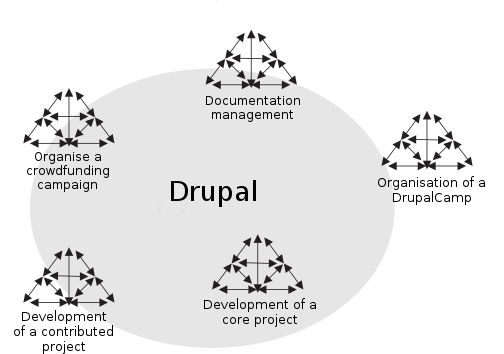
\includegraphics[scale=0.6]{diagrams/drupal_runaway_object.png}
	\caption[Conceptualisation of Drupal as a runaway object]%
	{Conceptualisation of Drupal as a runaway object. Based on figure \ref{engestrom-diagram-third-gen-b} of \textcite[306]{engestrom_future_2009}.}
	\label{drupal_runaway_object}
\end{figure}

As it will be shown in the next subsections, this enabled the analyses to be established at both the micro level of contribution activities, which is also the main unit of observation; as well as at the macro level, increasing the level of analysis to the study of the organisational environments which surround these contribution activities, since, as previously discussed, AT does not consider an a priori micro/macro divide \parencite{miettinen1999riddle}.

\subsection{Analysis at the micro level: exploring contribution activities}

For the analysis at the micro level, this study draws on the model of the activity system from the second generation of Activity Theory. More concretely, the notion of the human activity system is employed for the study of contribution activities. Commons-Based Peer Production communities focussed on digital commons, such as Drupal, typically rely on an economy of contribution \parencite{wittel2013counter}, around which their organisational life revolves. Hence, during the first stage of the research, it was necessary to study the notion of contribution\footnote{The findings regarding the study related to the notion of contribution in the case study are extensively presented and discussed in chapter \ref{identifyng-contribution:chapter}.} in itself within Drupal in detail, to broaden the understanding of contribution activities in FLOSS communities to those less visible. However, in order to understand how a large global community organises itself, it was necessary not only to acquire a better understanding of this notion of contribution, but also of the elements and factors (e.g. processes, dynamics and structures among others) which surround them.

Focussing on contribution activities, using the second generation of AT model as a lens, enabled the possibility to analyse some of these contribution activities in depth, including the relationships between the artefacts employed for collaboration, the roles played by its members (division of labour) and the implicit and explicit rules, among other entities from an AT perspective. Thus, as argued by \textcite{Uden2007}, the use of the activity system as a unit of analysis enables the incorporation of these notions as part of a dynamic phenomenon, avoiding simple monocausal explanations in the study of FLOSS. Furthermore, AT offers the advantage of performing historical analyses of the community behind it \parencite{Uden2007}, allowing a contextual study of  local practices and the emerging structures within it. For instance, how the rules have changed over time; or how they transited from implicit to explicit. In addition, it also facilitated the comparison between them, even when the main focus of action of these activities is of a different nature. For instance, while studying the development of code or the organisation of events.

An example of the application of the model of activity for the study of the development of \textit{contributed} projects\footnote{The different types of projects in the Drupal community are extensively discussed in chapter \ref{chapter:methods}.} in Drupal is depicted in figure \ref{drupal_module_at}, in which the elements of the activity were defined as follows:

\begin{itemize}
	\item \textit{Subject(s)}: the Drupalista(s) responsible for the development and maintenance of the \textit{contributed} project (maintainers).
	\item \textit{Mediating artefacts}: the coordination tools employed by the maintainers and the rest of the members of the community. A typical example of artefact are the issues lists associated to each project page in Drupal.org. They provide a means of interaction between the maintainers and the rest of the members of the community in which bugs can be reported, tasks can be assigned, or new functionalities can be requested, among other possibilities. It works also as a coordination tool for maintainers themselves. For instance, technical discussions about the different ways of implementing a functionality are often carried out using this artefact. Other types of artefacts are IRC channels, tools for directing messages between members of the community (via Drupal.org, e-mail or social networks such as Twitter) or Drupal discussion groups\footnote{\url{https://groups.drupal.org/}, accessed on \nth{13} January 2014.}.
	\item \textit{Object}: the project under constant development as a result of the activity.
	\item \textit{Rules}: they are the explicit and implicit rules which regulate the development of the project. Examples of explicit rules are the coding standards agreed by the community for projects\footnote{\url{https://drupal.org/coding-standards}, accessed on \nth{13} January 2014.} or the guidelines for contribution\footnote{\url{https://drupal.org/contribute/development}, accessed on \nth{13} January 2014.}. 	Examples of implicit rules are those employed by maintainers for the evaluation of contributions by Drupalistas without permission to make effective the proposed changes to the project.
	\item \textit{Community}: all the members of the Drupal community. The involvement in a concrete project is typically due to the fact that they are users of it. They can make use of mediated artefacts to provide feedback about it, patches to solve bugs or extend its functionalities, among others. 
	\item \textit{Division of labour}: represents the different roles typically associated with the distribution of tasks for the development of the project. An example of a form of division of labour is the allocation of tasks of development according to the different skills of the maintainers (backend developers, themers, user experience experts, etc.). The use of the issues list to allocate tasks between maintainers can be seen as a relationship between the division of labour and the artefacts.
\end{itemize}

\begin{figure}[H]
	\centering
	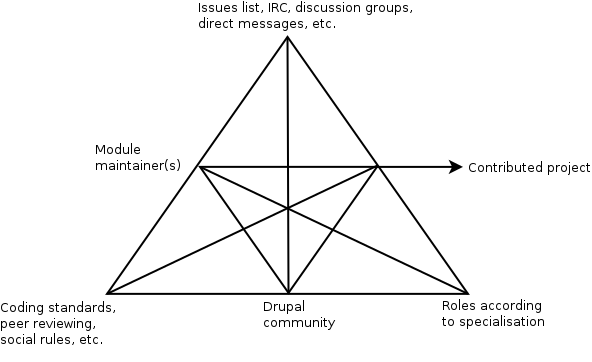
\includegraphics[height=8cm]{diagrams/drupal_module_at.png}
	\caption{Conceptualisation of the development of \textit{contributed} projects from an AT perspective.}
	\label{drupal_module_at}
\end{figure}

Similarly, the model of the activity system was employed for the study of different activities, such as the organisation of Drupal events\footnote{The different types of events in the Drupal community are extensively discussed in chapter \ref{chapter:methods}.}. For example, figure \ref{drupalcamp_at} provides an example of the application of the model in the organisation of a \textit{DrupalCamp}, a type of event organised by the community consisting of a conference typically lasting two or three days:

\begin{itemize}
	\item \textit{Subject(s)}: the participant(s) in the event.
	\item \textit{Mediating artefacts}: the coordination tools employed by the organisers and the rest of the members of the community. For example, the main website developed for the event, mailing lists or specific groups at Drupal.org.	
	\item \textit{Object}: the \textit{DrupalCamp} event.
	\item \textit{Rules}: the explicit and implicit rules which surround the event. Examples of explicit rules are the selection criteria for the presentations\footnote{See \url{http://2012.drupalcamp.es/en/node/23.html} (accessed on \nth{19} May 2015) for an example of speaker guidelines, in this case those used at \textit{DrupalCamp} Spain 2012.}, or codes of conduct\footnote{See \url{http://www.drupalcampbrighton.co.uk/content/code-conduct} (accessed on \nth{19} May 2015) for an example of a code of conduct, in this case that used at \textit{DrupalCamp} Brighton 2015.} outlining the shared ideals and values of the community. An example of implicit rules are social rules related to the reputation of a subject in the community and the power to carry out informal decision-making.
	\item \textit{Community}: all the members of the Drupal community.
	\item \textit{Division of labour}: the different roles of the participants during the event, for example, session reviewers, attendees or presenters.
\end{itemize}


\begin{figure}[h]
	\centering
	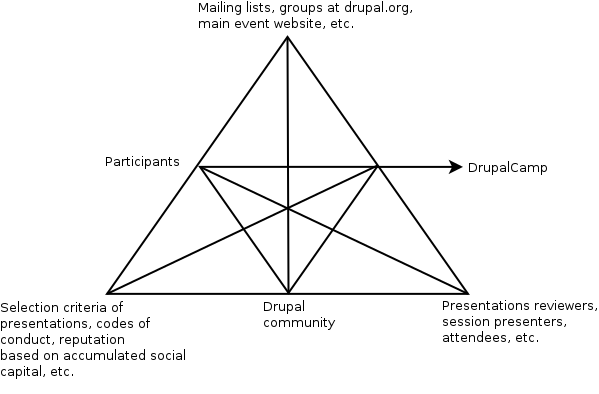
\includegraphics[height=8cm]{diagrams/drupalcamp_at.png}
	\caption{Conceptualisation of the participation in a \textit{DrupalCamp} from an AT perspective.}
	\label{drupalcamp_at}
\end{figure}

In addition, the use of Activity Theory for the analysis of contribution activities enables the incorporation of the concept of tension between the different entities which form part of the activity and its discovery while carrying out the analysis. For instance, regarding the first example of the development of a \textit{contributed} project, the tensions between designers and developers described by \textcite{Zilouchian2011} could be understood as an example of tension emerging from the division of labour, and it was then possible to study the impact of this tension on other entities of the model, such as rules. Similarly, for the example of the organisation of an event, this notion enabled the conceptualisation of how tensions related to having more objective and transparent procedures with regard to the selection of presentations (rules) affected the main artefacts of collaboration, provoking, for example, the inclusion of peer-reviewing systems to improve the transparency of the process.

\subsection{Analysis at a macro level: into the runaway object, or Drupal as a set of socio-technical systems}

As argued in the previous sections, the concepts of runaway object and human activity system enabled the analysis of some of the main challenges faced for the conceptualisation and study of organisational aspects in peer production. However, the pervasiveness \parencite[304-306]{engestrom_future_2009} of a runaway object, such as Drupal, provokes ambiguity in the position of the activity systems. As stated by \textcite[309]{engestrom_future_2009}, in peer production the ``boundaries and structures of activities systems seem to fade away", however, this mode of production requires and creates ``bounded hubs of concentrated coordination efforts" \parencite[310]{engestrom_future_2009}, which is the way in which the new generation of Activity Theory approaches these challenges. Hence, in order to connect the micro and macro aspects which surround this case study, this research required the exploration of these bounded hubs in order to shed light on how a large global CBPP community such as Drupal organises itself. However, while the model of the human activity system remains valuable for the study of CBPP communities such as Drupal, and the concept of runaway object operates as a nexus allowing them to connect micro and macro, this study required a more precise definition of what these ``bounded hubs of concentrated coordination efforts" are.

For these reasons, in this study, the concept of \textit{socio-technical systems of contribution} has been created, developed and employed for the study of Commons-Based Peer Production communities, such as Drupal. This concept draws on the Socio-Technical Systems approach from organisational theory \parencite{trist1981evolution}, providing a more accurate definition of what these bounded hubs of coordination efforts are in CBPP. By \textit{socio-technical}, the aim is to emphasise the interrelatedness between the social and the technical aspects of the organisation in these communities. By incorporating the term \textit{contribution}, the concept encompasses the relevance which this notion has in these communities, as previously outlined in chapter \ref{chapter:introduction}. Hence, the notion of a socio-technical system of contribution from which this study develops was defined as:

\textsl{A set of interacting parts, including people, software, hardware, procedures or rules among others, which form a complex whole that revolves around networks of human activity systems which are perceived as contribution within the community and share a similar main focus of action.}

For example, while the development of a \textit{contributed} Drupal project is, as previously presented, conceptualised as a human activity system from an Activity Theory perspective, the network of thousands of \textit{contributed} modules in Drupal.org can be conceptualised as a socio-technical system of contribution within the community. Similarly, while the model of human activity system was employed for the analysis of the organisation of a \textit{DrupalCamp}, the network of \textit{DrupalCamps} is conceptualised as a socio-technical system of contribution.  Figure \ref{STSoC}, provides an illustration of the application of this concept, in which the human activity systems are grouped according to the socio-technical system they belong to. The illustration also shows how the human activities within these groups are interconnected, as well as showing interactions between different socio-technical systems of contribution within the runaway object of Drupal.

\begin{figure}[h]
	\centering
	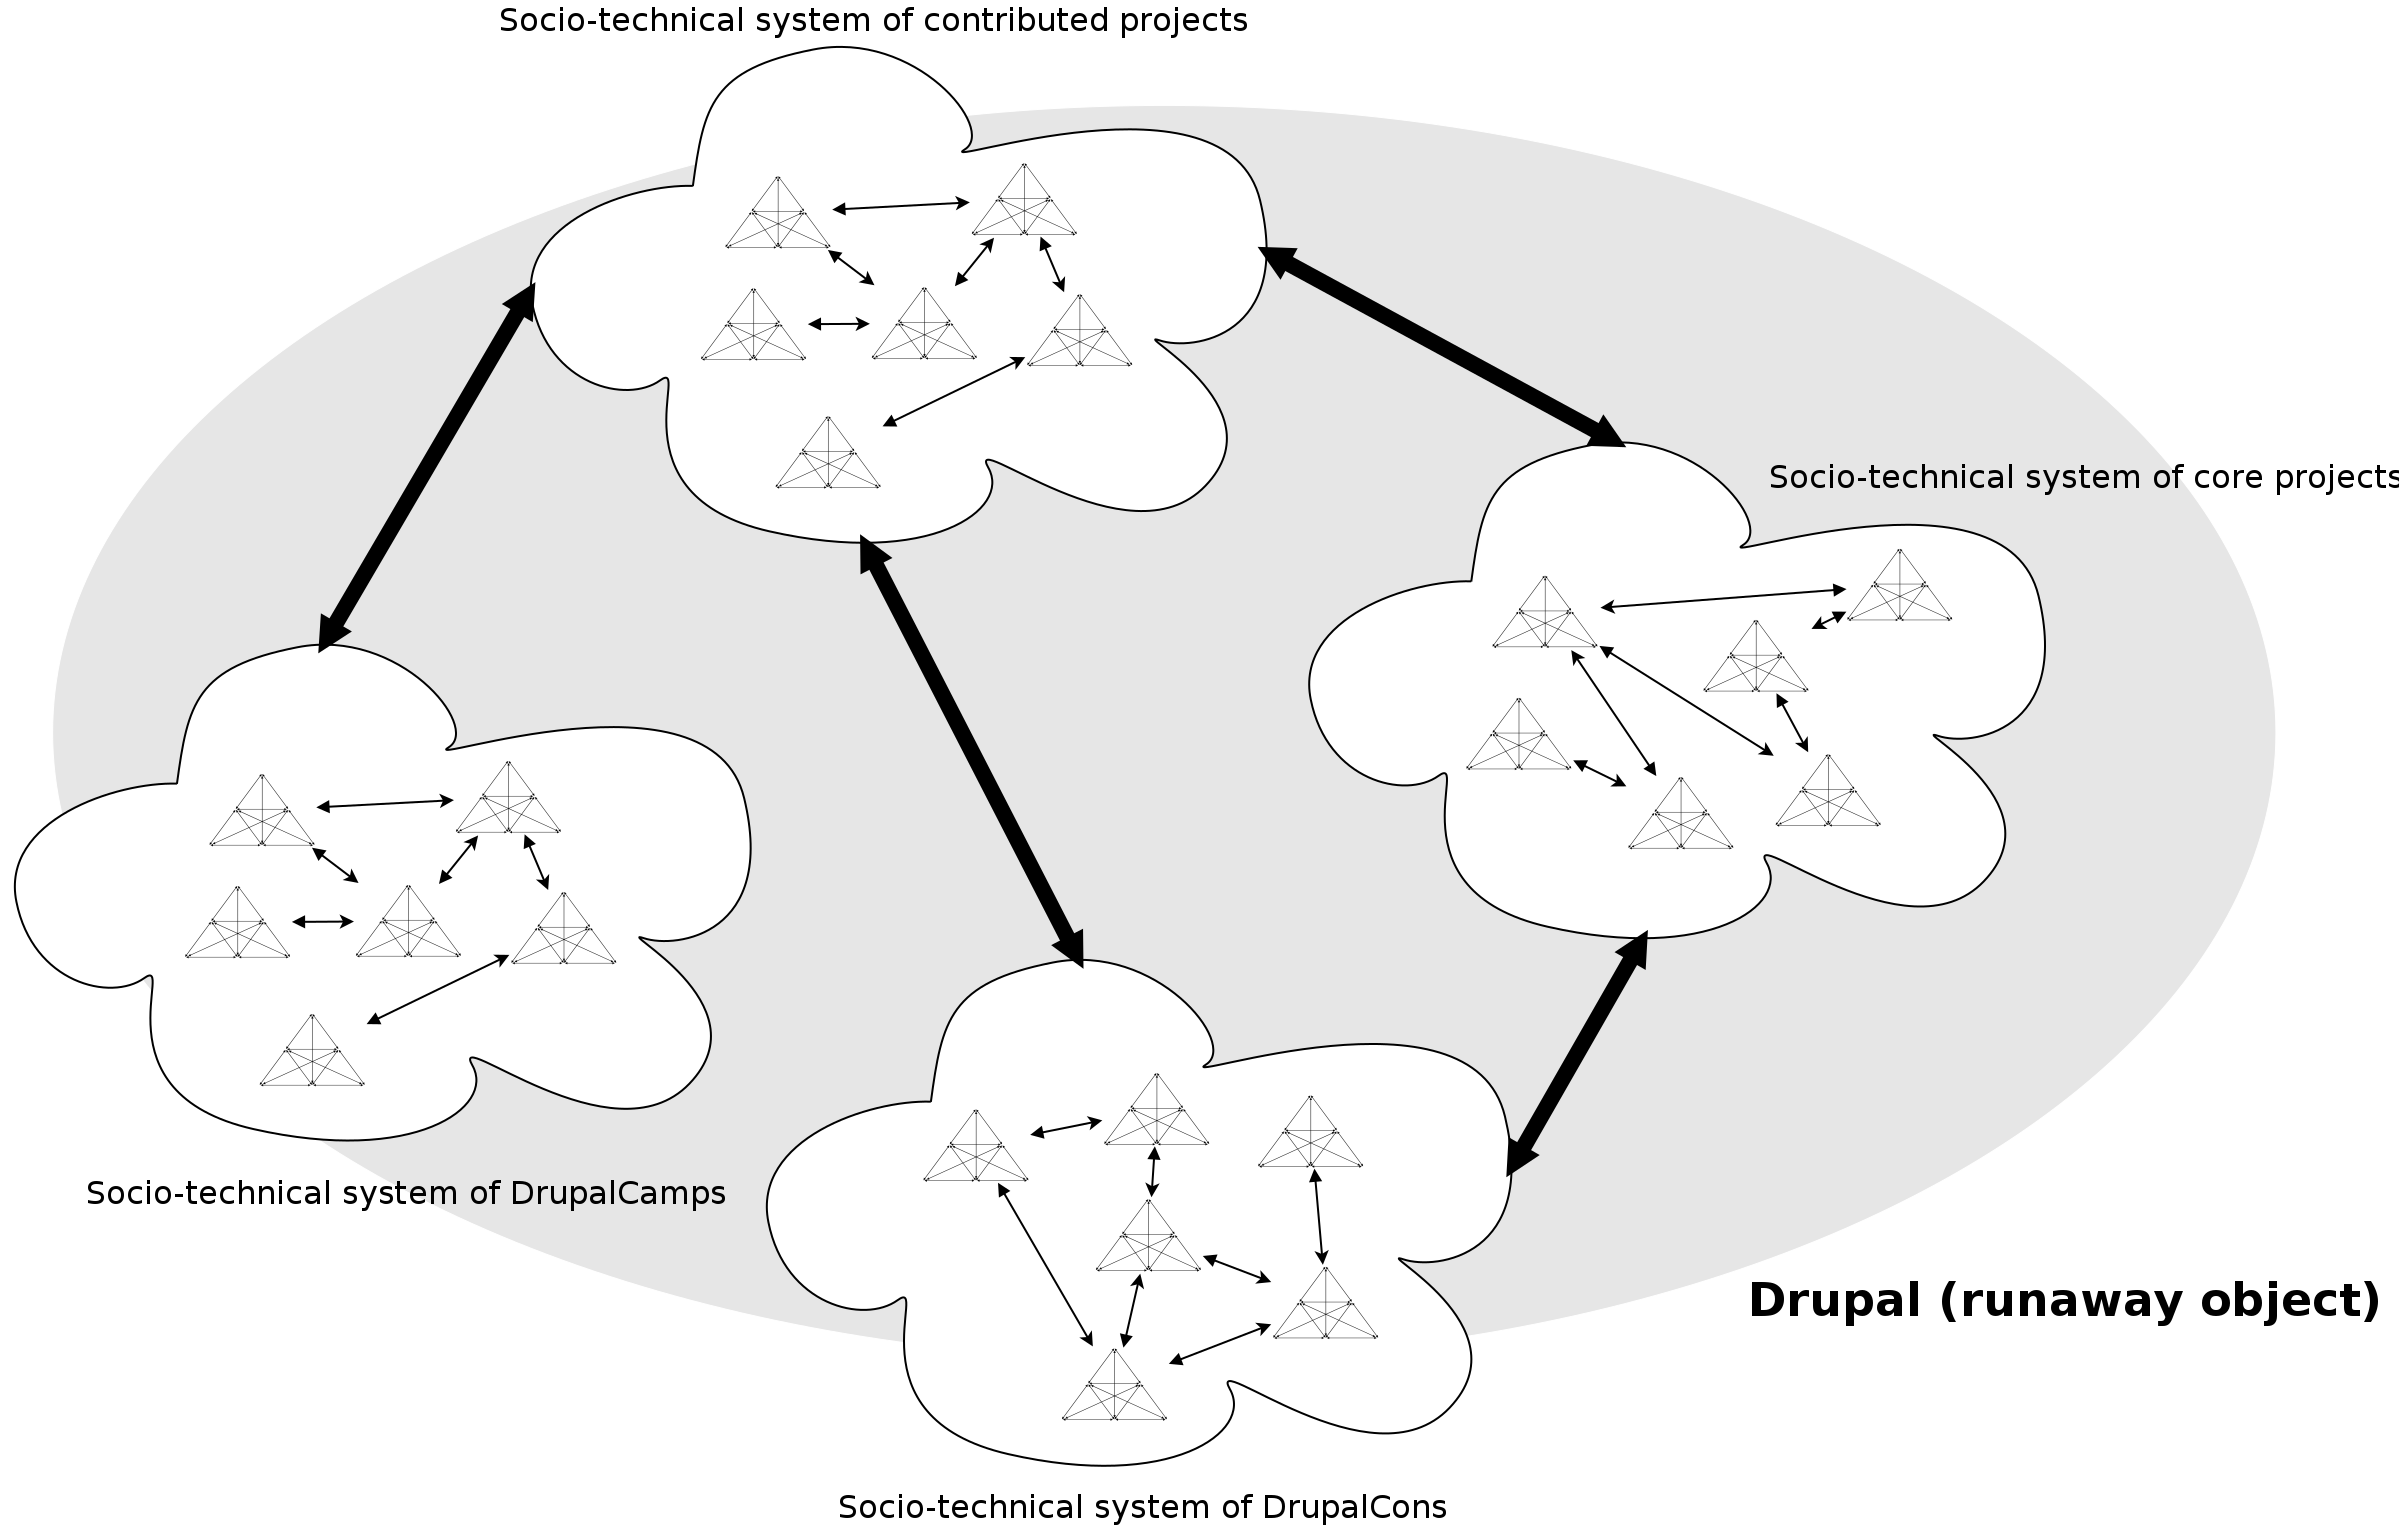
\includegraphics[height=10cm]{diagrams/STSoC.png}
	\caption[Conceptualisation of Drupal as a set of socio-technical systems of contribution]{Conceptualisation of Drupal (runaway object) as a set of socio-technical systems of contribution.}
	\label{STSoC}
\end{figure}

Thus, in a similar way as defining contribution activities as a main unit of analysis, this enables the exploration not only of the object, but also the entities which surround the activity and the tensions between them; the notion of socio-technical systems of contribution enabled their connection to the macro levels at which they occur, as well as the tensions between different socio-technical systems of contribution. Hence, this concept draws on the notion of bounded hubs of coordination from the third generation of Activity Theory, but provides a more precise definition according to the characteristics of Commons-Based Peer Production communities. As discussed in section \ref{subsec:why-at}, the necessity to provide a more accurate definition is in line with the undergoing efforts of activity theorists to rethink the third generation of Activity Theory to accommodate the changes in organisation towards a network society \parencite{castells2011rise}, characterised by a distributed workforce and the predominance of knowledge work, as also in the case of peer production. Hence, the analysis presented in chapters \ref{sec:custom-to-contrib} to \ref{mostly-offline-cons:chapter}, is focussed not only on the workings of contribution activities themselves (micro level), but also on the interactions between the networks they form as socio-technical systems of contribution, and how these socio-technical systems of contribution emerged, evolved, interact with each other, and were shaped by different organisational dynamics (macro level).


\section{Conclusion}
\label{sec:at-conclusion}

The lack of clear boundaries and the distributed nature of peer production represents a challenge for the application of theoretical frameworks for its study. However, it was concluded that Activity Theory provided an appropriate tool for the conceptualisation and analysis of this case study. Firstly, the ambivalence of the boundaries in peer production is acknowledged by the new generation of Activity Theory, providing a degree of flexibility to adapt the theoretical framework to the context of the case study, and thus allowing a more precise definition when necessary due to the specific context of the case study: socio-technical systems of contribution. Secondly, the use of the model of activity as a unit of analysis helped in defining those boundaries, while also playing an important role in reconsidering the notion of contribution activities in these communities. Thirdly, AT facilitated the analysis and comparison of the organisational dynamics, the relationships between entities, their tensions and outcomes, for significantly diverse but key contribution activities identified in the study. In this way, the understanding of Drupal as a runaway object operates as a nexus for them. Thus, it facilitated the conceptualisation of Drupal as shared by all these contribution activities, despite the diversity of the subjects carrying them out, the multi-faceted nature of its medium and the intermittent nature of the hubs of collaboration in peer production.

In this way, it was concluded that Activity Theory is a valuable tool for the study of the organisational processes of contribution activities, allowing the main objective to be explored: to improve our understanding of how large and global CBPP communities, such as Drupal, organise themselves.